\documentclass{article}

\usepackage{fullpage}
\usepackage{url}
\usepackage{graphicx}
\usepackage{subcaption}
\usepackage{amsmath}
\usepackage{physics}
\usepackage{pxfonts}
\usepackage{mathtools}
\usepackage{float}
\usepackage{placeins}

\DeclareMathOperator{\erfi}{erfi}
\newcommand{\R}{\ensuremath{\mathbb{R}}}

\title{Statistical Mecahincs I Excercise 3}
\author{Idan Stark}
\date{\today}

\begin{document}
\maketitle

\section{2D Lattice Gauge Theory}
\subsection{Low temperature expansion of the dual 3D Ising model}
The Dual 3D Ising model is the 3D model where the spins sit on the edges of the lattice and not the vertices, and interact via the plaquette they sit on. In other words, four spins interact in each plaquett:
\begin{equation}
    H = -J\sum_{plaquettes}\sigma^P_1\sigma^P_4\sigma^P_3\sigma^P_4
\end{equation}
Where $P$ is the index of the plaquette and the lower indices are the specific spin on the plaquette. We saw in class that the high-temperature expansion of this model is dual to the lower temperature expansion of the 3D Ising model. We shall now show that the low temperature expansion of this model is also dual to the high temperature expansion of the Ising model.
\newline
The low temperature expansion is done by starting from a groun state where all spins are either up or down. The partition function at temperature zero is:
\begin{equation}
    Z_{T=0} = 2^{N+1} e^{12NK}
\end{equation}
Where the factor $2$ comes from the two options - all spins down and all spins up - and the factor $2^N$ comes from the gauge symmetry of the model, i.e. changing the spins on all edges touching a specific vertex will not change the total energy of the system. In general, we will take this factor for all terms in the expansion. The factor 12 in the exponent comes from each spin being a part of four plaquettes, and that there are $3N$ plaquettes in the model.
\newline
Now let us look for the smallest possible increments in energy. The three contenders are the flipping of one, two spins that share a plaquette, and three spins that share a vertex.
\newline
Let us start with one spin. This will flip the four plaquettes that include it, adding $8K$ to the total energy. There are $3N$ such spins to flip: 3 edges for each vertex in the lattice.
\newline 
Next let us look at two spins that share a plaquette. To see why this is the lowest energy increment coming from two spins, let us see all our options. Flipping two spins can be either on the same plaquette or not on the same plaquette. On different plaquettes, this is the same as flipping one spin twice, and so adds $16K$ to the energy.
On the other hand, If they share a plaquette, then they flip it twice, and so only the six plaquettes that they do not share flip. In this case the energy increment will be $12K$. It can be seen then that the more plaquettes the spins share, the less their combined energy increment will be. There are $3N$ plaquettes in the lattice, each of them there are $\binom{4}{2} = 6$ combinations of spins, therefore there are $18N$ such possible flips, which must also be reduced from the next step.
\newline
Lastly, let us attempt to flip three spins that share a vertex. We look at this case because the spins share the biggest amount of plaquettes, and so the energy increment in it will be minimal. Each of the three spins shares two of its plaquettes with another spin and has two additional plaquettes. All shared plaquettes flip twice, and so the effect cancels, and only the six unshared plaquettes flip. The energy increment is then $12K$, similar to two spin flip. There are $N$ vertices in the lattice, each of them includes four configurations for the positions of the flipped spins - 2 options for each direction are $2^3 = 8$ options, divided by 2 to remvoe the double counting, since each two opposite configurations are a gauge transformation apart, and we already accounted for it in the $2^N$ factor. The energy increments and their multiplicities are summarized in the table \ref{tab:energy_increments}.
\begin{table}[h]
    \centering
    \begin{tabular}{|c|c|c|}
        \hline
        Flipped spins & Energy increment & Multiplicity \\
        \hline
        1 & $8K$ & $3N$ \\
        \hline
        2 (sharing a plaquette) & $12K$ & $18N$ \\
        \hline
        3 (sharing a vertex) & $12K$ & $4N$ \\
        \hline
    \end{tabular}
    \caption{Energy increments and multiplicities for low temperature expansion of the dual 3D Ising model.}
    \label{tab:energy_increments}
\end{table}
The low temperature expansion is then
\begin{equation}
    Z_{cold} = 2^{N+1} e^{12NK}\left(
        1 + 3N e^{8K} + 22N e^{12K} + \cdots
    \right)
\end{equation}
For comparison, the high temperature expansion of the 3D Ising model is:
\begin{equation}
    Z_{high} = 2^N \cosh(K)^{3N}\left(
        1 + 3N e^{4T} + 22N e^{6T} + \cdots
    \right)
\end{equation}
Which shows that these two models are dual to each other.
\subsection{The gauge transformation in 2D}
Just like in the 3D case, the 2D case has a gauge symmetry: Flipping the spins on all four edges coming from a single vertex will cause each plaquette between them to be flipped twice, thus the total energy will stay the same. We can use this transformation to show that any configuration is energetically equivilant to a configuration in which all the horizontal spins are $\uparrow$ (calling $\uparrow = 1$ and $\downarrow = -1$ and ignoring the edges).
\newline
First, let us notice that whenever there are two neighbooring $\downarrow$ spins, we can flip the vertex between them, flipping the vertical spins while changing the horizontal spins to $\uparrow$. This means that for every uninterrupted chain of spins that are all $\downarrow$, we can flip them in pairs until none are left if the length of the chain is even and one left if the length of the chain is odd:
\begin{equation*}
\begin{gathered}
    \uparrow\downarrow\downarrow\downarrow\downarrow\uparrow\uparrow \longrightarrow 
    \uparrow\uparrow\uparrow\downarrow\downarrow\uparrow\uparrow \longrightarrow 
    \uparrow\uparrow\uparrow\uparrow\uparrow\uparrow\uparrow
    \\
    \uparrow\downarrow\downarrow\downarrow\downarrow\downarrow\uparrow \longrightarrow 
    \uparrow\uparrow\uparrow\downarrow\downarrow\downarrow\uparrow \longrightarrow 
    \uparrow\uparrow\uparrow\uparrow\uparrow\downarrow\uparrow
\end{gathered}
\end{equation*}
Second, let us notice that we can "shift" single spins along the horizontal direction by flipping one of the vertices it touches:
\begin{equation*}
    \uparrow\downarrow\uparrow\uparrow\uparrow\uparrow\uparrow \longrightarrow 
    \uparrow\uparrow\downarrow\uparrow\uparrow\uparrow\uparrow \longrightarrow 
    \uparrow\uparrow\uparrow\downarrow\uparrow\uparrow\uparrow
\end{equation*}
These two operations - "removing" pairs of spins and "shifting" a single spin along the line - allow us to "remove" all horizontal down spins. We simply "shift" the spins at the edges of groups one by one until they all touch eachother, then cancle all of them out. Examples:
\begin{equation*}
\begin{gathered}
    \uparrow\uparrow\downarrow\downarrow\downarrow\downarrow\uparrow\uparrow\downarrow\uparrow\downarrow\downarrow\downarrow \ \overset{shift}{\longrightarrow} \
    \uparrow\uparrow\uparrow\uparrow\uparrow\downarrow\downarrow\downarrow\downarrow\downarrow\downarrow\downarrow\downarrow \ \overset{remove}{\longrightarrow} \
    \uparrow\uparrow\uparrow\uparrow\uparrow\uparrow\uparrow\uparrow\uparrow\uparrow\uparrow\uparrow\uparrow
    \\
    \downarrow\uparrow\downarrow\uparrow\uparrow\downarrow\uparrow\uparrow\downarrow\uparrow\downarrow\downarrow\downarrow \ \overset{shift}{\longrightarrow} \ 
    \uparrow\uparrow\uparrow\uparrow\uparrow\uparrow\downarrow\downarrow\downarrow\downarrow\downarrow\downarrow\downarrow \ \overset{remove}{\longrightarrow} \ 
    \uparrow\uparrow\uparrow\uparrow\uparrow\uparrow\uparrow\uparrow\uparrow\uparrow\uparrow\uparrow\downarrow
\end{gathered}
\end{equation*}
\newline
There is a caviet to this method. As can be seen in the second example above, in the case where a horizontal row has an odd number of spins, one spin will remain at the end. This spins can be pushed to the edge where it be neglected, or, if the lattice has open boundary conditions, the gauge symmetry at the edge allows flipping it without flipping another horizontal spin, since at the edge there are only two plaquettes touching the vertex.
\subsection{Solving the model in 2D}
So, every state is energetically equivilant to another state with all horizontal spins up. This means that writing the partition function we can group the states by this equiliance relation, simply mulplying the partition function by the multiplicity of the horizontal line, and use the energy of the all-horizontal-spins-up state as the hamiltonian for all of the equivilant states:
\begin{equation}
    Z = 2^{N_H} \sum_{\{\sigma_i\}} \prod_{plaquette} \exp[K\sigma_1^P\sigma_2^P]
\end{equation}
Where $N_H$ is the number of horizontal spins and $\sigma_1^P$ and $\sigma_2^P$ are the vertical spins in each plaquette. Now, this remainds us of the 1D Ising model, but there is still a caviet - there are $N_H$ chains, not one. But, since the they do not interact, and since they are idendical, we get:
\begin{equation}
    Z = N_H 2^{N_H} \sum_{\{\sigma_i\}} \prod_{\langle i,j \rangle} \exp[K\sigma_i\sigma_j]
\end{equation}
Which is exactly the 1D Ising model, up to a constant the will be remove by normalization. The value of the partition function is, using the developed in class using the transfer matrix method:
\begin{equation}
    Z = N_H 2^{N_H + N_V} \cosh^{N_V}(K)
\end{equation}

\section{Umbrella Sampling in the 1D Ising Model}
Let us consider the 1D Ising model with periodic boundary conditions:
\begin{equation}
    H(\{\sigma_i\}) = -J \sum_{i=1}^N \sigma_i \sigma_{i+1}
\end{equation}
with $J = 1$ and $N = 128$. At a temperature of $T = 2.5$ the magnetization distribution $P(m)$ is sharplu peaked around $m = 0$. In this section we exmaine numeric evaluation methods for the distribution using Umbrella sampling.
\subsection{Direct sampling}
First, let us look at a direct sample. To do this, we ran a standard Monte-Carlo simulation with single-spin Metropolis dynamics. We ran the simulation with twnety samples running simultaniously. The system was first allowed to reach convergence. Convergence is defined by two criteria, and is considered reached only when both are met. The first is for the standard diviation of the averages of the twenty samples along the last ten repetitions to be under a threshold, defined to be 1. The second condition is for the slope of the average of the twenty samples along the last ten repetitions to be below a threshold defined to be 0.001. These two conditions measure convergence and stability, respectivly.
\newline
After reaching convergence, the simultion ran over the twenty samples for an additional 1000 sweeps, using these 20,000 samples (20 samples over 1000 sweeps) as the population for the distribution. This distribution can be seen in figure \ref{fig:direct-sampling}\footnote{The code for this section can be found in \url{https://raw.githubusercontent.com/idanstark42/masters-homework/refs/heads/master/sm1/ex3/umbrella_sampling_1D_Ising.py}}.
\begin{figure}[H]
    \centering
    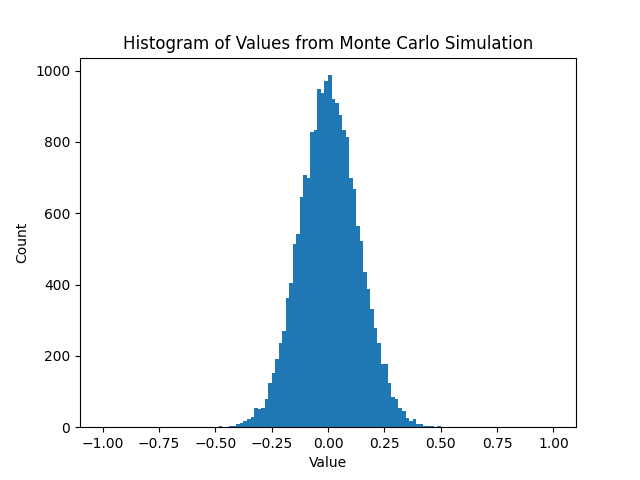
\includegraphics[width=0.7\textwidth]{monte_carlo_histogram_20260104_230724.png}
    \caption{Histogram of magnetization values from direct sampling of the 1D Ising model at $T = 2.5$.}
    \label{fig:direct-sampling}
\end{figure}
The system reached convergence after twelve sweeps. It can be seen in the figure that the distribution is sharply peaked around $m = 0$, and that the tails of the distribution are very poorly sampled, with only a few samples in the ranges $|m| > 0.5$. In reality, only one sample was found in the range $|m| > 0.5$, and so the histogram bar is not visible in the figure.
\newline
This was expceted, since at high temperatures the spins are disordered, leading to a magnetization probability peak around zero.
\subsection{Using Umbrella potential}
Now let us add the umbrella potential:
\begin{equation}
    H_U = H + W(m) \qquad W(m) = \frac{k}{2}(m-m_0)^2
\end{equation}
with $k = 2000$\footnote{The question required $k = 200$, but after a trial it did not move the center to $0.6$, only to $0.4$. This is due to the bias not being strong enough against the original hamiltonian, the entropy and the high temperature pushing the magnetization to the center a non-negligble amount. To bypass this and see the full effect of the Umbrella potential, I used a bias one order of magnitude higher.} and $m_0$ = 0.6. The new distribution can be seen in figure \ref{fig:umbrella-potential}. It can be seen that the new center of the distribution is $m = 0.6$.
\begin{figure}[H]
    \centering
    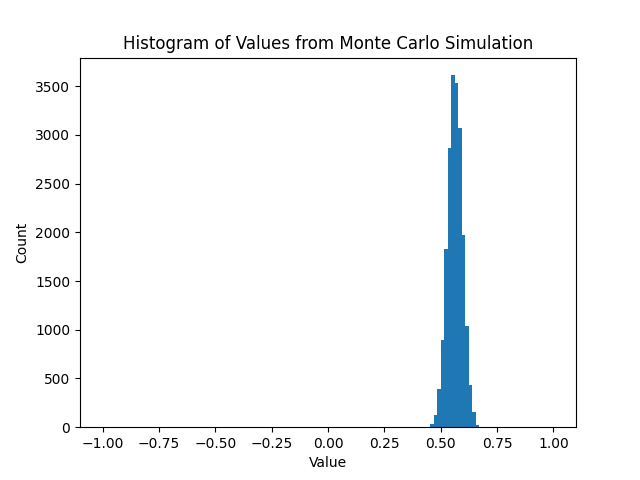
\includegraphics[width=0.7\textwidth]{monte_carlo_histogram_20260104_231207.png}
    \caption{Histogram of magnetization values from Umbrella sampling of the 1D Ising model at $T = 2.5$ with umbrella potential centered at $m_0 = 0.6$.}
    \label{fig:umbrella-potential}
\end{figure}
\subsection{The umbrella sampling identity}
As we saw in class, the actual probability $P(m)$ of a variable over a hamiltonian $H$ can be related to a new hamiltonian $H_U = H + W$ using:
\begin{equation}
    P(m) = e^{-\beta H(m)} = e^{-\beta H_U(m)}e^{\beta W(m)} = P_U(m)e^{\beta W(m)}
\end{equation}
This allows us to evaluate $P(m)$ using a modified hamiltonian, not having the same numerical sampling biases as the original hamiltonian. In our case, we can remove the bias we gained in the previous subsection. The new distribution after removing the bias can be found in figure \ref{fig:umbrella-potential-after-correction}. It can be seen that this time the distribution is not a full gaussian, but rather only the right tail. In order to compare it to \ref{fig:direct-sampling}, let us normalize both distributions and plot them together, as can be seen in figure \ref{fig:direct-vs-umbrella}.
The unbiased umbrella distribution was thus renormalized to have the same maximum. This was achieved using a truncated gaussian fit on the biased umbrella distribution, finding the theoretical maximum of the gaussian, and then dividing the distribution by the ratio between the maxima. In addition, the exact solution has been added and normalized in the same way. Notice that it was done for comparison, and that the gaussian is not meant to be a fit for any of the distributions.
\newline
The main difference, it seems, is that in in the unbiased umbrella distribution $P_{US}(m)$, there are much more samples in the $|m| > 0.5$ region, even after removing the bias. While both of them are, unsurprisingly, gaussians, and thus fitting to the theoretical exact solution, it is clear from the exact solution in the graph that they are both unpercise in their distribution.
\subsection{Discussion}
It seems that the umbrella simultion is a useful tool to investigate parts of the distribution that are usually noisy. The potential acts as a harmoic potential, changing the center of the distribution and the region it samples. This helps remove noises that may occour from low volume of samples. In our case, the umbrella simultion sampled $m \approx 0.6$ because the potential was the lowest there. Later mulplying the distribution by the factor $e^{\beta W(m)}$ removed the bias, since as we saw, it is the bridging potential between the direct and biased potentials, and so it is mathematically equivilant while computationally it helps reduce the noises stemming from the small number of samples in the region when preforming direct sampling. In total, we get a process that moves the center of the distribution to an area that was previously mostly noise, getting enough samples in that are to have statistically significant results, and then using the physical relation between the direct and biased distributions to go back to the original distribution center, now with the larger number of samples in the previously unsampled region.

\begin{figure}[H]
    \centering
    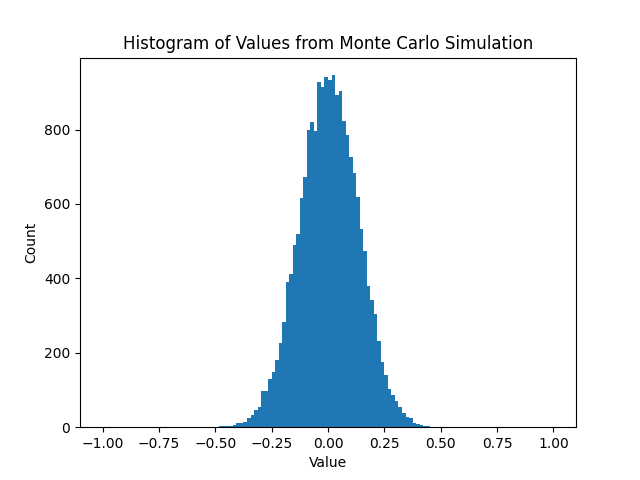
\includegraphics[width=0.7\textwidth]{monte_carlo_histogram_20260104_231732.png}
    \caption{Histogram of magnetization values from Umbrella sampling of the 1D Ising model at $T = 2.5$ with umbrella potential centered at $m_0 = 0.6$, after removing the bias using the umbrella sampling identity.}
    \label{fig:umbrella-potential-after-correction}
\end{figure}
\begin{figure}[H]
    \centering
    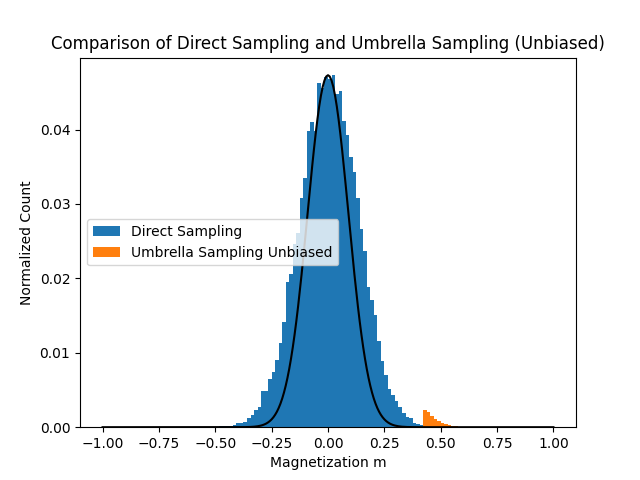
\includegraphics[width=0.7\textwidth]{direct_vs_umbrella_20260105_042624.png}
    \caption{Histogram of magnetization values from the unbiased Umbrella sampling and the direct sampling, after normalization to a simialr maximum.}
    \label{fig:direct-vs-umbrella}
\end{figure}

\section{Yang-Lee zeros of the 1D Ising model}
\subsection{Rewriting the partition function}
The parition function of the 1D Ising model can be written using the transfer matrix method:
\begin{equation}
    Z_N = \lambda_{+}^N + \lambda_{-}^N
\end{equation}
Where
\begin{equation}
    \lambda_{\pm} = e^{\beta J}\cosh(\beta B) \pm \sqrt{e^{2\beta J}\cosh^2(\beta B) - 2\sinh(2\beta J)}
\end{equation}
Defining:
\begin{equation}
    \rho = e^{-2 \beta B} \qquad \tau = e^{-2 \beta J}
\end{equation}
Then:
\begin{equation}
\begin{gathered}
    e^{\beta J}\cosh(\beta B) = \frac{1}{\sqrt{\tau}}\frac{\frac{1}{\sqrt{\rho}} + \sqrt{\rho}}{2} = \frac{1 + \rho}{2\sqrt{\rho\tau}}
    \\
    e^{2\beta J}\cosh^2(\beta B) = \left(\frac{1 + \rho}{2\sqrt{\rho\tau}}\right)^2 = \frac{1 + 2\rho + \rho^2}{4\rho\tau}
    \\
    2\sinh(2\beta J) = e^{2\beta J} - e^{-2\beta J} = \frac{1 - \tau^2}{\tau}
\end{gathered}
\end{equation}
We get:
\begin{equation}
    \lambda_{\pm} = \frac{1 + \rho}{2\sqrt{\rho\tau}} \pm \sqrt{\frac{1 + 2\rho + \rho^2}{4\rho\tau} - \frac{1 - \tau^2}{\tau}} = \frac{1 + \rho \pm \sqrt{\left(1 - \rho\right)^2 + \left(2\tau\right)^2\rho}}{2\sqrt{\rho\tau}}
\end{equation}
So:
\begin{equation}
    Z = \left(\frac{1 + \rho + \sqrt{\left(1 - \rho\right)^2 + \left(2\tau\right)^2\rho}}{2\sqrt{\rho\tau}}\right)^N + \left(\frac{1 + \rho - \sqrt{\left(1 - \rho\right)^2 + \left(2\tau\right)^2\rho}}{2\sqrt{\rho\tau}}\right)^N
\end{equation}
\subsection{Numerically solving the equation}
Let us now find the values $\rho$ for which $Z = 0$:
\begin{equation}
    \left(\frac{1 + \rho + \sqrt{\left(1 - \rho\right)^2 + \left(2\tau\right)^2\rho}}{2\sqrt{\rho\tau}}\right)^N + \left(\frac{1 + \rho - \sqrt{\left(1 - \rho\right)^2 + \left(2\tau\right)^2\rho}}{2\sqrt{\rho\tau}}\right)^N = 0
\end{equation}
Moving $\lambda_{-}$ to the other side
\begin{equation}
    \left(\frac{1 + \rho + \sqrt{\left(1 - \rho\right)^2 + \left(2\tau\right)^2\rho}}{2\sqrt{\rho\tau}}\right)^N = - \left(\frac{1 + \rho - \sqrt{\left(1 - \rho\right)^2 + \left(2\tau\right)^2\rho}}{2\sqrt{\rho\tau}}\right)^N
\end{equation}
Then dividing by it
\begin{equation}
    \left(\frac{1 + \rho + \sqrt{\left(1 - \rho\right)^2 + \left(2\tau\right)^2\rho}}{1 + \rho - \sqrt{\left(1 - \rho\right)^2 + \left(2\tau\right)^2\rho}}\right)^N = - 1
\end{equation}
And taking the $N$-th root:
\begin{equation}
    \frac{1 + \rho + \sqrt{\left(1 - \rho\right)^2 + \left(2\tau\right)^2\rho}}{1 + \rho - \sqrt{\left(1 - \rho\right)^2 + \left(2\tau\right)^2\rho}} = e^{i\pi (2k+1)/N}
\end{equation}
We get a quadratic equation for $\rho$. To solve it, let us multiply by the denominator, and move everything such that the root is isolated:
\begin{equation}
    1 + \rho + \sqrt{\left(1 - \rho\right)^2 + \left(2\tau\right)^2\rho} = e^{i\pi (2k+1)/N} \left(
        1 + \rho - \sqrt{\left(1 - \rho\right)^2 + \left(2\tau\right)^2\rho}
    \right)
\end{equation}
\begin{equation}
    \left(
        e^{i\pi (2k+1)/N} + 1\right)\sqrt{\left(1 - \rho\right)^2 + \left(2\tau\right)^2\rho}
     =  \left(e^{i\pi (2k+1)/N} - 1\right)\left(
        1 + \rho
    \right)
\end{equation}
\begin{equation}
    \sqrt{\left(1 - \rho\right)^2 + \left(2\tau\right)^2\rho}
     =  \frac{e^{i\pi (2k+1)/N} - 1}{e^{i\pi (2k+1)/N} + 1}\left(
        1 + \rho
    \right)
\end{equation}
Now, it's easy to see:
\begin{equation}
    \frac{e^{i\pi (2k+1)/N} - 1}{e^{i\pi (2k+1)/N} + 1} = \frac{e^{i\pi (2k+1)/2N} - e^{i\pi (2k+1)/2N}}{e^{i\pi (2k+1)/2N} + e^{i\pi (2k+1)/2N}} = i\tan(\frac{2k+1}{2N}\pi) \equiv i\alpha_k
\end{equation}
And so, we get:
\begin{equation}
    \sqrt{\left(1 - \rho\right)^2 + \left(2\tau\right)^2\rho}
     = i\alpha_k\left(
        1 + \rho
    \right)
\end{equation}
\begin{equation}
    \left(1 - \rho\right)^2 + \left(2\tau\right)^2\rho
     = -\alpha_k^2\left(1 + \rho\right)^2
\end{equation}
\begin{equation}
    \rho^2 - 2\rho + 1 + 4\tau^2\rho
     + \alpha_k^2\rho^2 + 2\alpha_k^2\rho + \alpha_k = 0
\end{equation}
\begin{equation}
    (1 + \alpha_k^2)\rho^2 + (4\tau^2 - 2 + 2\alpha_k^2)\rho + (1 + \alpha_k^2)
     = 0
\end{equation}
\begin{equation}
    \rho^2 + \frac{4\tau^2 - 2 + 2\alpha_k^2}{1 + \alpha_k}\rho + 1
     = 0
\end{equation}
And so we got a quadratic equation for $\rho$. Solving it will give the values of $\rho$ for which $Z = 0$. Figure \ref{fig:zeros-of-z-different-n} shows the zeros on the complex plain for $N = 10, 50, 500$ and $\tau = 0.5$\footnote{The code for this calculation can be found in \url{https://raw.githubusercontent.com/idanstark42/masters-homework/refs/heads/master/sm1/ex3/yang_lee_zeros_1D_ising.py}}.
\begin{figure}[ht]
  \centering
  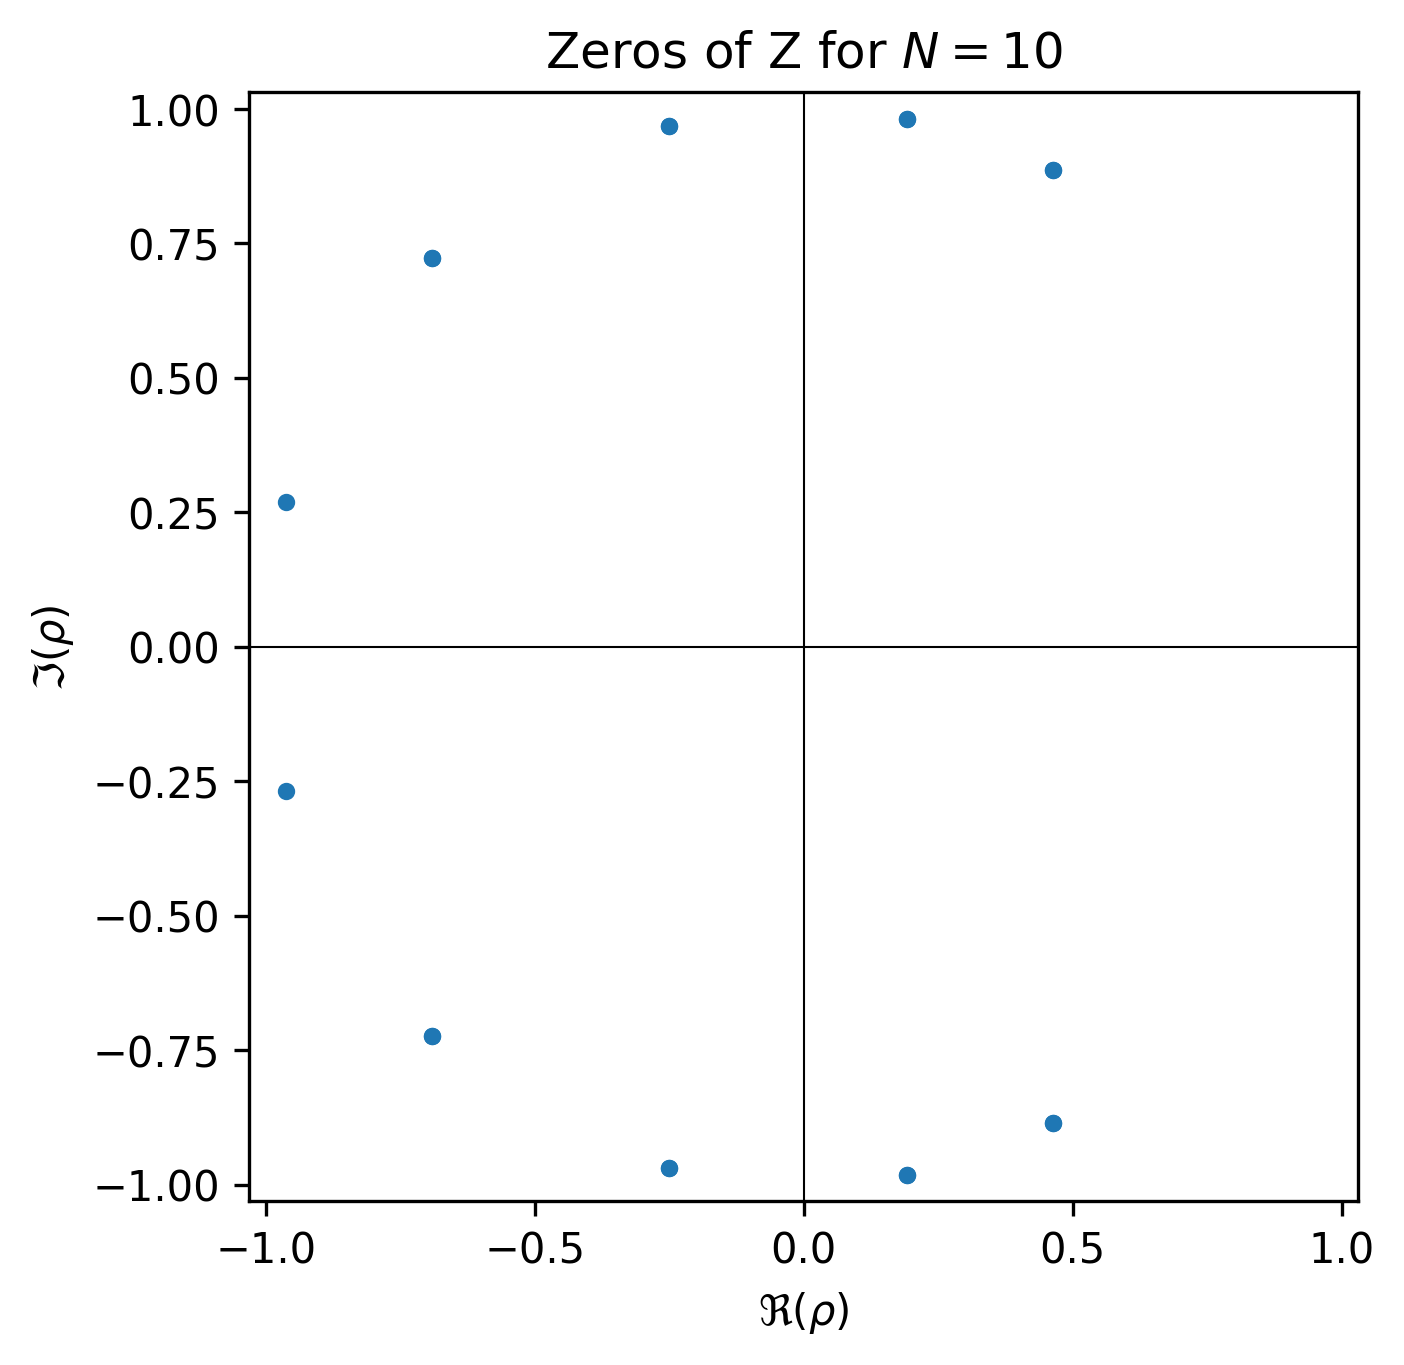
\includegraphics[width=0.3\textwidth]{rho_scatter_N10.png} \hspace{0.02\textwidth}
  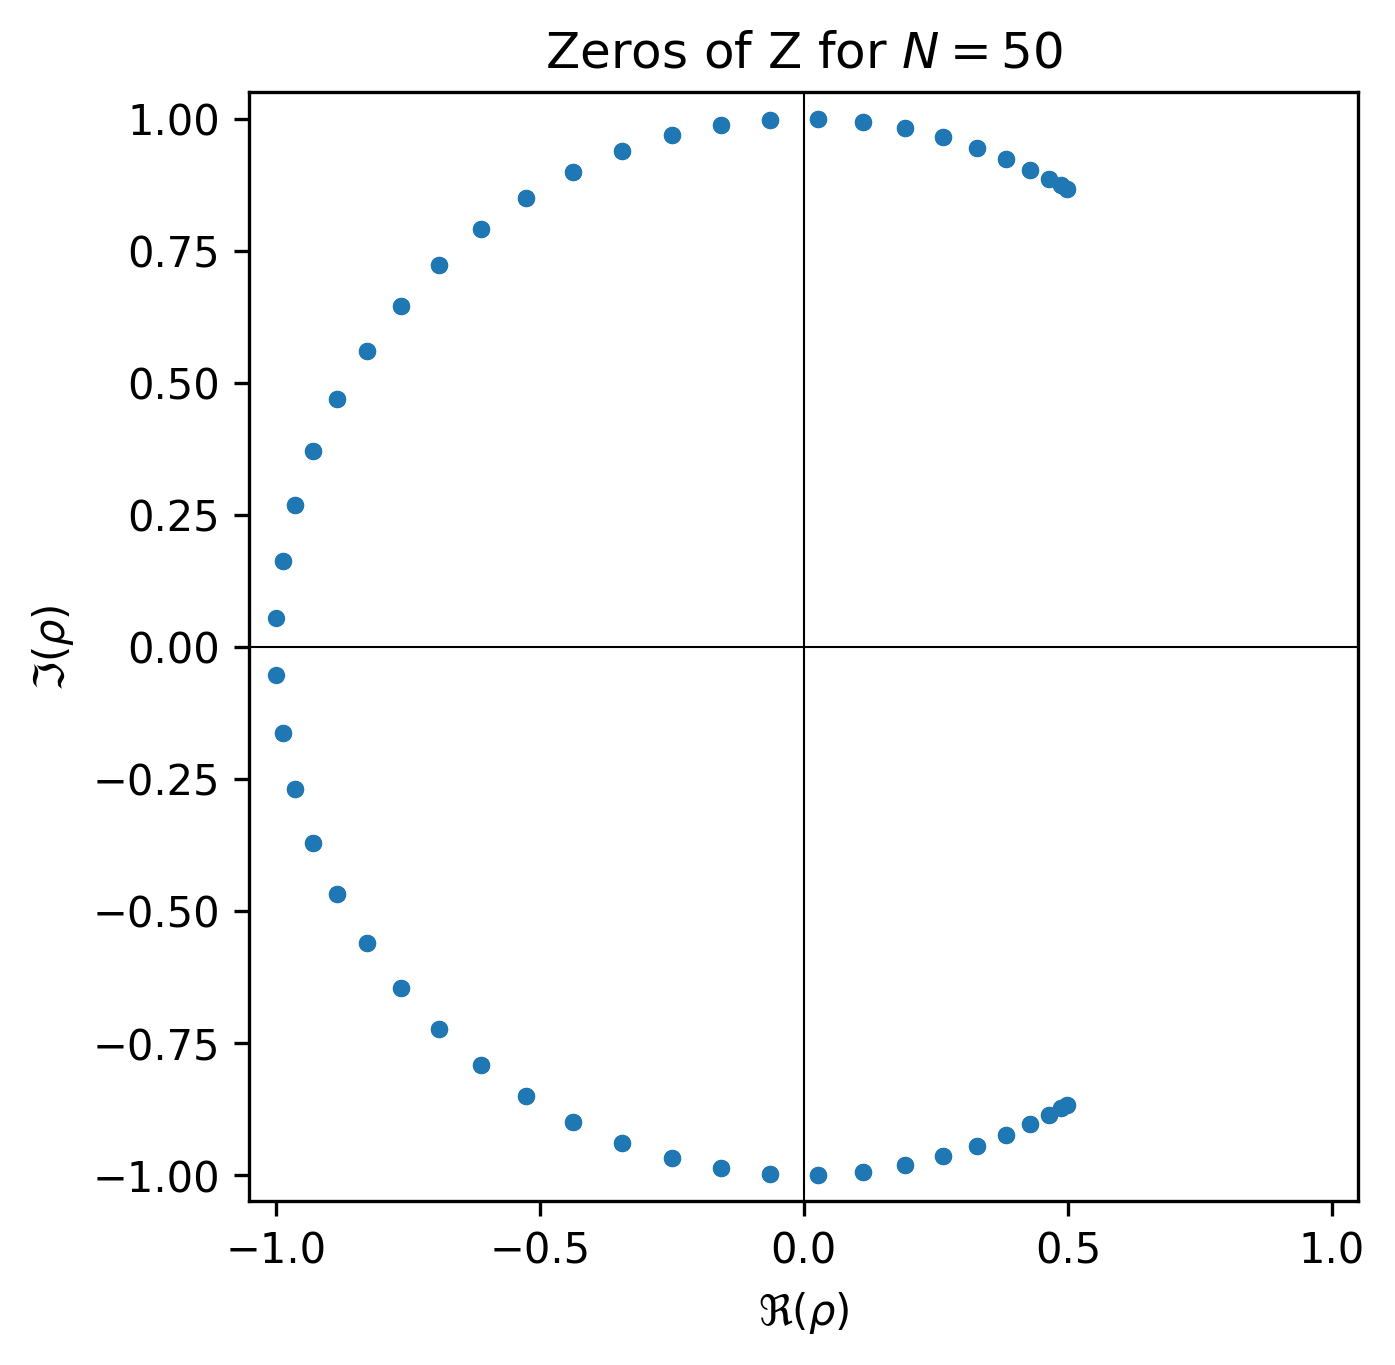
\includegraphics[width=0.3\textwidth]{rho_scatter_N50.png} \hspace{0.02\textwidth}
  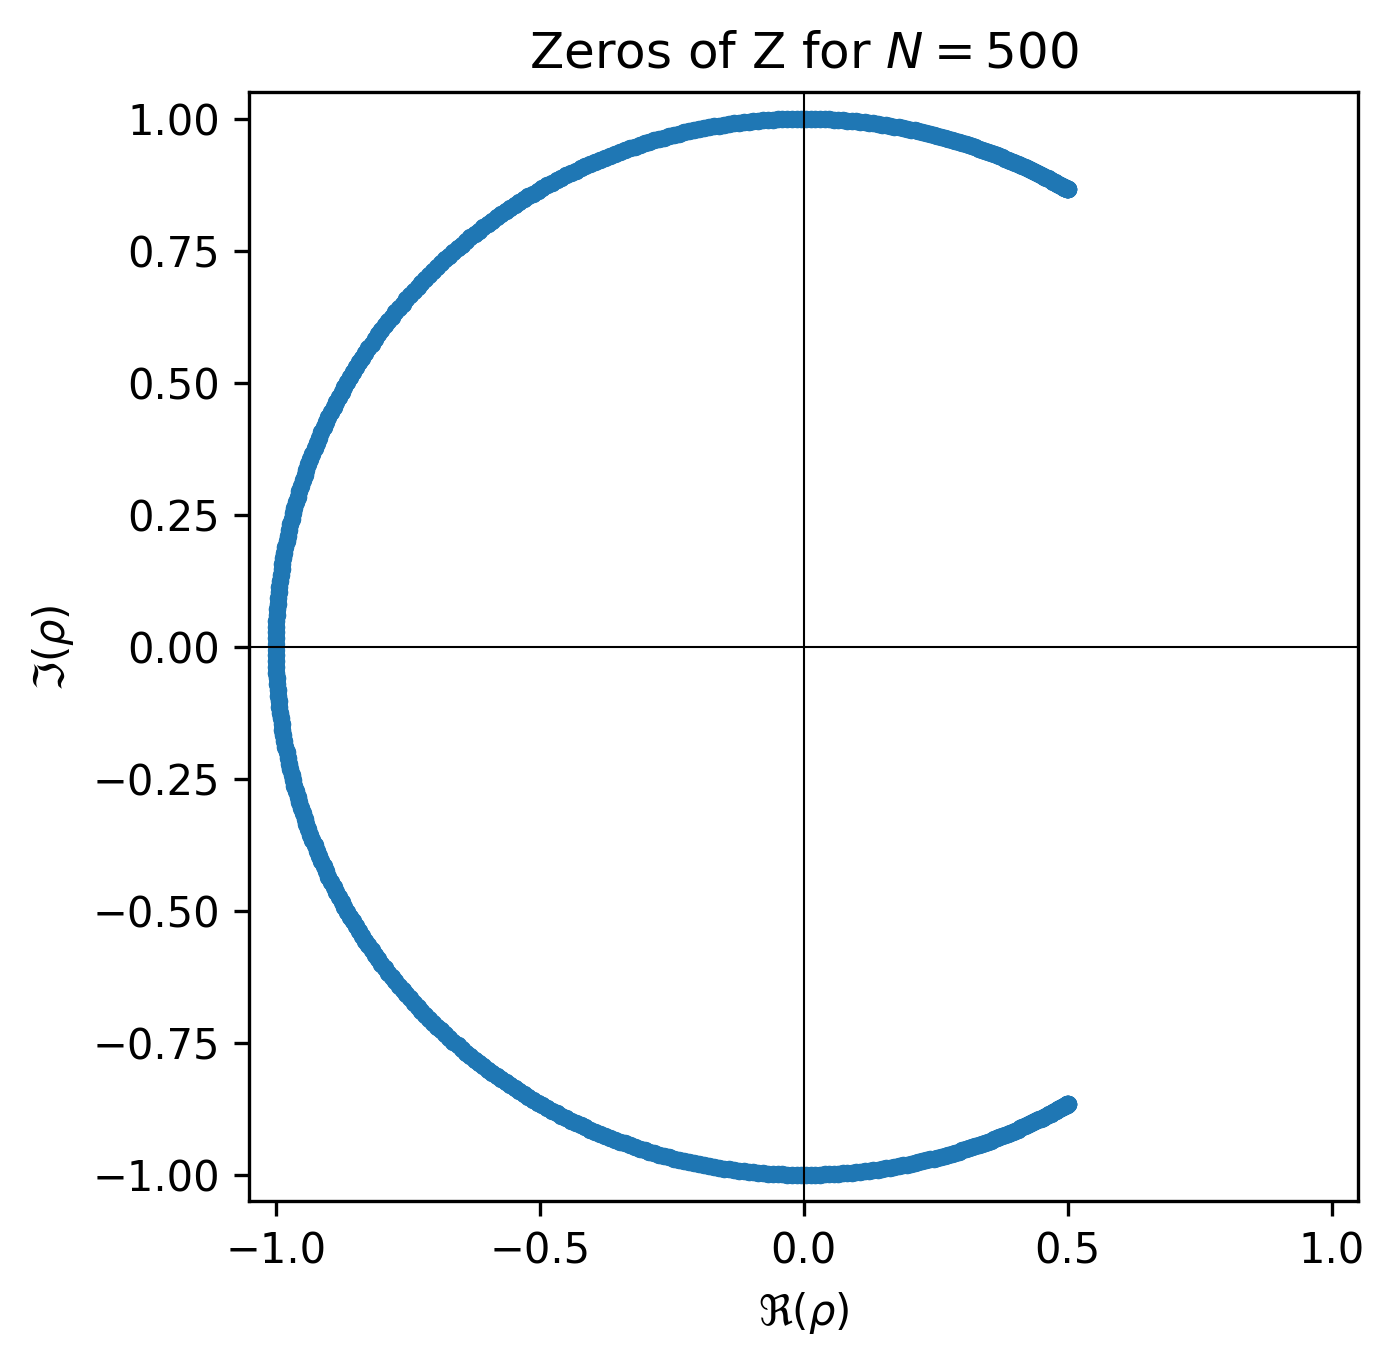
\includegraphics[width=0.3\textwidth]{rho_scatter_N500.png}
  \caption{Complex values of $\rho$ for which $Z = 0$ for $N = 10, 50, 500$ (from left to right) and $\tau = 0.5$}
  \label{fig:zeros-of-z-different-n} % <- after caption
\end{figure}
\begin{figure}[ht]
  \centering
  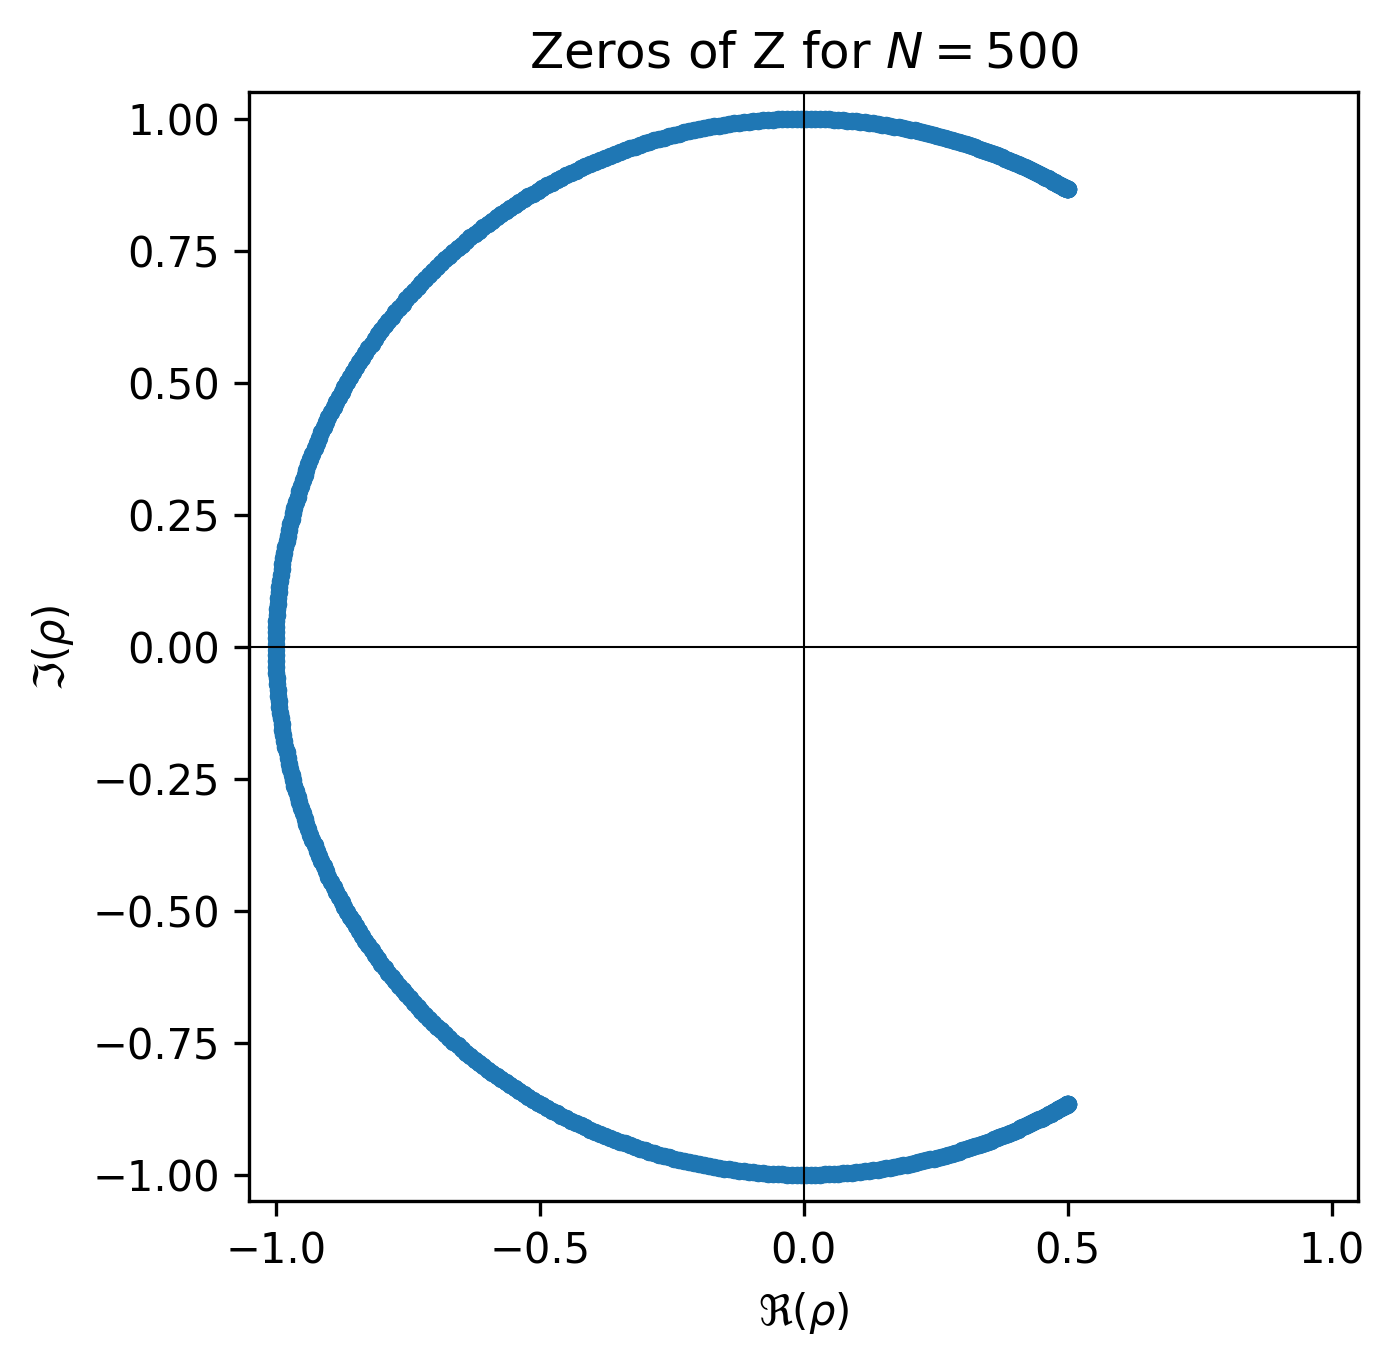
\includegraphics[width=0.3\textwidth]{rho_scatter_N500.png} \hspace{0.02\textwidth}
  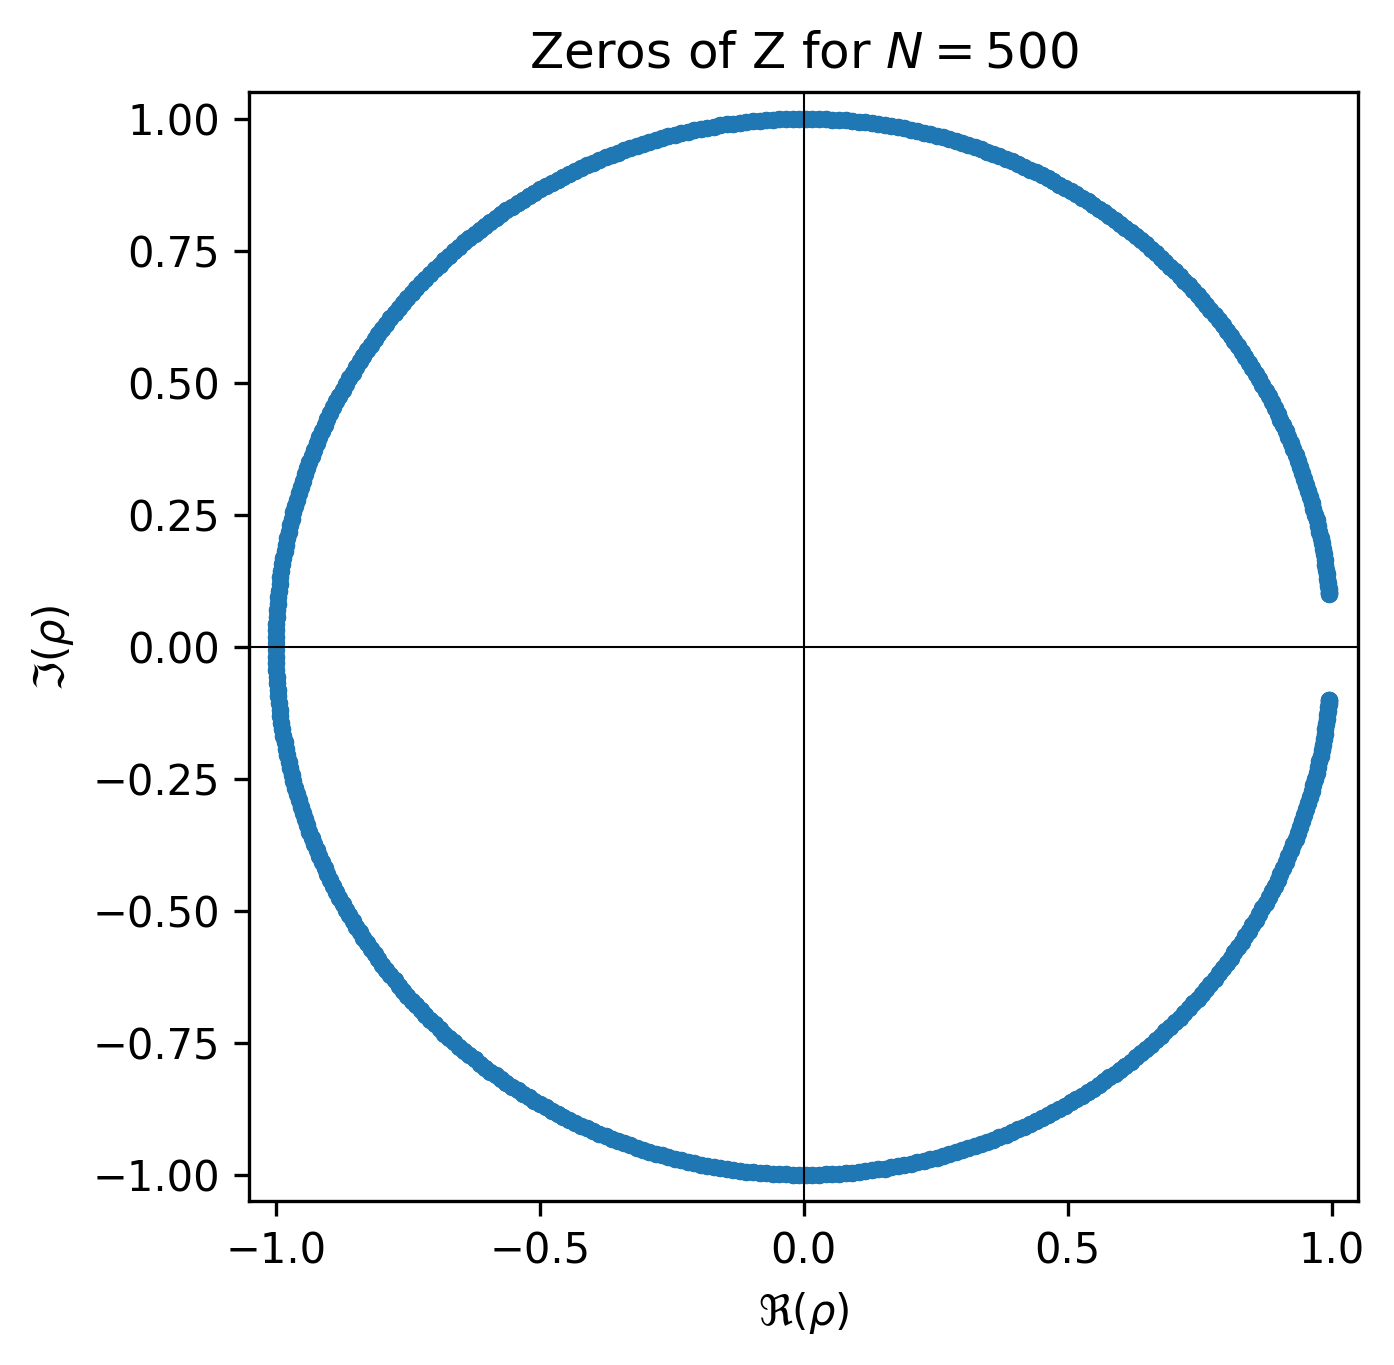
\includegraphics[width=0.3\textwidth]{rho_scatter_N500_tau_0.05.png} \hspace{0.02\textwidth}
  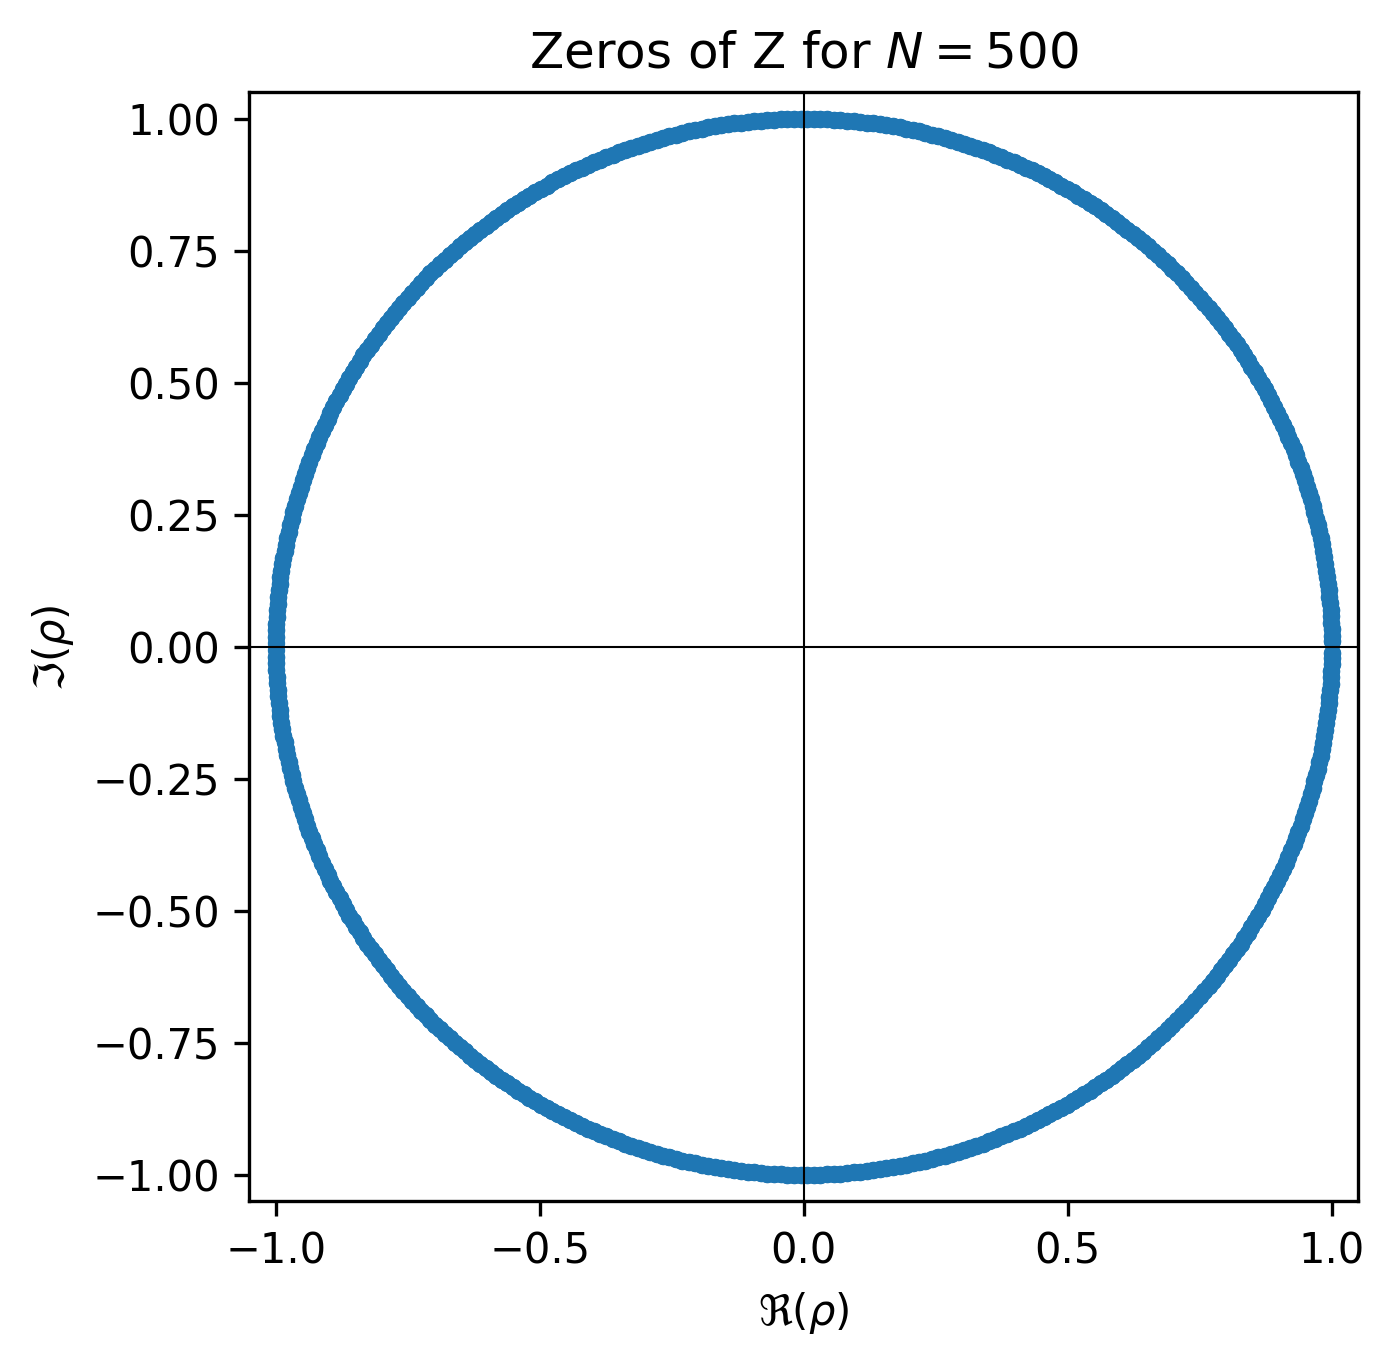
\includegraphics[width=0.3\textwidth]{rho_scatter_N500_tau_0.005.png}
  \caption{Complex values of $\rho$ for which $Z = 0$ for $N = 500$ and $\tau = 0.5, 0.05, 0.005$ (from left to right)}
  \label{fig:zeros-of-z-different-taus} % <- after caption
\end{figure}

\subsection{Very high $\beta$}
Let us look at the regieme where $\beta \rightarrow \infty$, or in other words, $T \rightarrow 0$. We expect there to be a phase transition in the system where sufficient $B$, or in other words, sufficiently small $\rho$, will cause the system to move between the two ground states - all spins up and all spins down. From the symmetry of the system, it is expected that the transition will be at $B = 0$.
\newline
According to Yang-Lee theory, the value of $\rho$ for which such transition will occour is the value on the real axis where the zeros of the partition function are condensed as $N \rightarrow \infty$. In our case, increasing $\beta$ is mathematically equivilant to decreasing $\tau$. The values of $\rho$ for which $Z=0$ for different values of $\tau$ are visible in figure \ref{fig:zeros-of-z-different-taus}. It can be seen that the closer $\tau$ is to zero, the closer the points are to touching on the positive side of the real axis, at $\rho = 1$, as expected.
\end{document}